\documentclass[letter, 10pt]{article}
\usepackage[utf8]{inputenc}
\usepackage[spanish]{babel}
\usepackage{amsfonts}
\usepackage{amsmath}
\usepackage[top=3cm,bottom=3cm,left=3.5cm,right=3.5cm,footskip=1.5cm,headheight=1.5cm,headsep=.5cm,textheight=3cm]{geometry}
\usepackage{listings}
\usepackage{color}
\usepackage{graphicx}
\usepackage{hyperref}

\begin{document}
%\pagestyle{empty}


\title{Bioinformática\\``Tarea Anotación de Genomas''}
\author{Rodrigo Fernández \and Cristián Maureira \and Gabriel Zamora\\\texttt{\{rfernand,cmaureir,gzamora\}@inf.utfsm.cl}}
\date{\today}
\maketitle

\section{Problema}
Investigue como funciona el algoritmo CYK y de que
forma puede ser extendido para las gramáticas de contexto
libre probabilísticas. Debe entregar un reporte de una
página con sus conclusiones y opcionalmente una página
extra para anexos (imágenes, gráficos, etc…)
%Links de Ayuda
%http://www-tsujii.is.s.u-tokyo.ac.jp/~tsuruoka/papers/ijcnlp04.pdf
%link2

\section{Algoritmo CYK}
% de la wikipedia: http://es.wikipedia.org/wiki/Algoritmo_CYK
En términos más simples, la función principal del algoritmo es considerar todas las posibles
subsecuencias de una secuencia de palabras determinadas y poder establecer $P[i, j, k]$ a verdadero
si es que la subsecuencia de palabras que empiezan desde $i$ de longitud $j$ puede ser generada desde $R_k$.

Estando consideradas las subsecuencias que posean una longitud $1$, se
continúa con las subsecuencias que tengan longitud $2$, y así sucesivamente.

Para las subsecuencias de longitud 2 o mayor, el algoritmo considera cada posible
partición de la subsecuencia en dos partes, comprobando si existe alguna regla $P \rightarrow Q R$
en la que $Q$ concuerda con la primera parte y $R$ con la segunda.

Si se cumple, se establece que $P$ concuerda con la subsecuencia completa.

Una vez se complete este proceso,
la frase será reconocida por la gramática si es que la subsecuencia que contiene la frase completa concuerda
con el símbolo inicial utilizado.

\section{Algoritmo CYK y gramáticas de contexto}
% de la wikipedia: http://es.wikipedia.org/wiki/Algoritmo_CYK
Es posible poder extender el \emph{algoritmo CYK} para analizar ``cadenas'' usando
\emph{gramáticas libres de contexto con pesos} y \emph{gramáticas libres de contexto
probabilísticas}.

Los \emph{pesos} o \emph{probabilidades} serán almacenados en la tabla $P$ en
vez de los valores booleanos utilizados anteriormente.

De esta manera $P[i, j, A]$ contendrá el mínimo
peso (máxima probabilidad) de que la subcadena desde $i$ hasta $j$ pueda ser
derivada por $A$.

Otras extensiones permiten al algoritmo enumerar todos los
posibles análisis de una frase ordenándolos de menor a mayor peso (mayor a
menor probabilidad).

%\section{Conclusiones}
% información sobre gramática libre de contexto probabilistica:
%http://es.wikipedia.org/wiki/Gram%C3%A1tica_libre_de_contexto_probabil%C3%ADstica

\newpage
\section{Anexos}

\begin{center}
    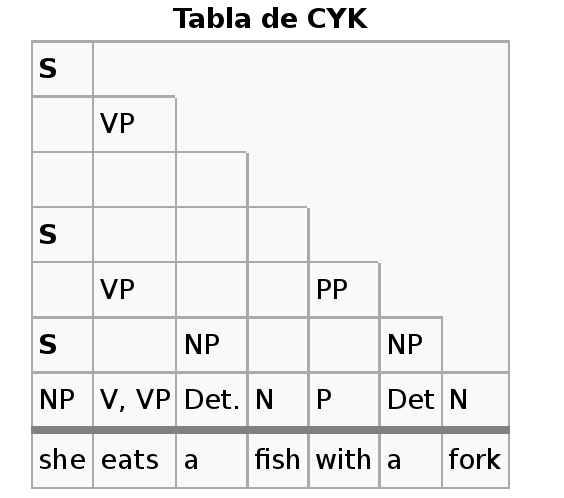
\includegraphics[width=0.6\textwidth]{cyk_table}
\end{center}
\lstset{ %
language=Pascal,                % choose the language of the code
basicstyle=\footnotesize,       % the size of the fonts that are used for the code
numbers=left,                   % where to put the line-numbers
numberstyle=\footnotesize,      % the size of the fonts that are used for the line-numbers
stepnumber=1,                   % the step between two line-numbers. If it's 1 each line 
                                % will be numbered
numbersep=5pt,                  % how far the line-numbers are from the code
backgroundcolor=\color{white},  % choose the background color. You must add \usepackage{color}
%keywordstyle=\color{blue}\bfseries,
showspaces=false,               % show spaces adding particular underscores
showstringspaces=false,         % underline spaces within strings
showtabs=false,                 % show tabs within strings adding particular underscores
frame=true,                   % adds a frame around the code
tabsize=2,                  % sets default tabsize to 2 spaces
captionpos=b,                   % sets the caption-position to bottom
breaklines=false,                % sets automatic line breaking
breakatwhitespace=false,        % sets if automatic breaks should only happen at whitespace
caption="Algoritmo CYK",             % also try caption instead of title
escapeinside={\%*}{*)},         % if you want to add a comment within your code
morekeywords={*,...}            % if you want to add more keywords to the set
}

\lstinputlisting{CYK_algorithm}



\vfill\hfill
RF/CM/GZ/\LaTeX
\end{document} 
